\subsection{3D Rectification}


\begin{figure}[h!]
  \centering
  \resizebox{0.45\textwidth}{!}{
  \resizebox{0.8\textwidth}{!}{\minipage{0.3\textwidth}
      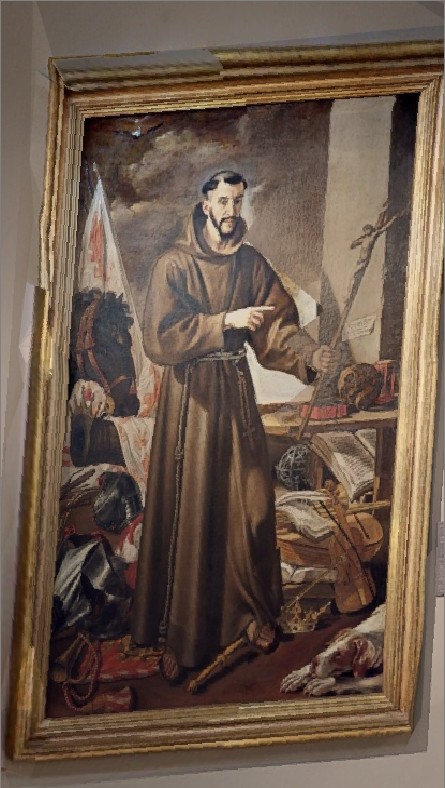
\includegraphics[width=\linewidth]{pictures/painting_detection/3d_rectification_original.PNG}
      \caption*{Original 3D model painting}\label{fig:rectification_original}
    \endminipage\hfill}
    \resizebox{0.8\textwidth}{!}{\minipage{0.3\textwidth}
      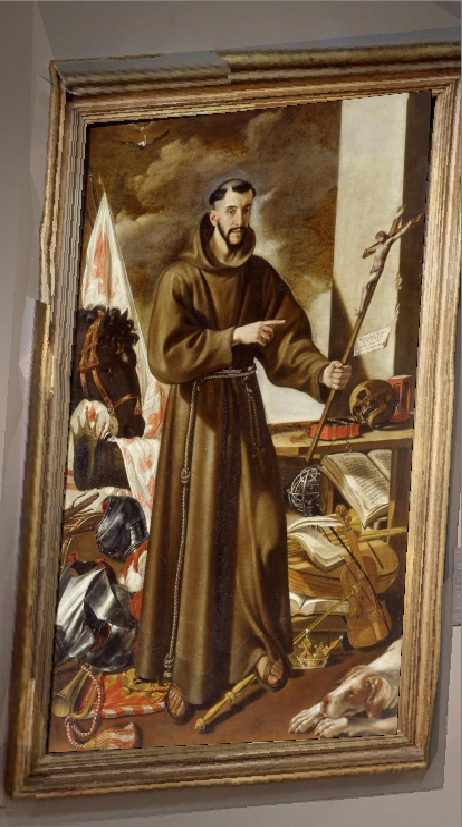
\includegraphics[width=\linewidth]{pictures/painting_detection/3d_rectification_warped.PNG}
      \caption*{Replaced painting}\label{fig:rectification_warped}
    \endminipage\hfill}}
    \caption{Painting rectification from the 3D view.}\label{fig:3d-warping}
\end{figure}


The 3D Rectification is the last optional task we've been achieved. The goal was to replace the painting from a 3D model's view with the same painting but with an higher resolution, retrieved from the database. Given some screenshots from the 3D model, we identify, through our trained network, all the paintings ROIs and each of them is compared with all the paintings in the database. The retrieved painting is first warped with an homographic trasformation, in order to be in the same perspective of the painting in the screenshot, and then it is replaced instead of the original painting. If the painting is not found, the warping is not performed. An example of our approach is shown in fig.~\ref{fig:3d-warping}.

